\chapter{GraphQL}
\section{Typ-System}

Das GraphQL-Typ-System wird zur Definierung eines Schemas verwendet.
Ein Schema beschreibt einen GraphQL-Service und besteht aus den abrufbaren Ressourcen, ihren Relationen zueinander und ihren Interaktionsmöglichkeiten.


Eine eingehende Anfrage wird durch die im Schema definierte Datenstruktur validiert.
Wenn die in der Anfrage enthaltene Query durch das Typ-System erfolgreich validiert wurde, wird die beinhaltete Operation an die Implementierung weitergeleitet.
Dafür zerlegt GraphQL die übergebene Query und gibt sie an den jeweiligen Resolver weiter. Diese Resolver interagieren mit der Geschäftslogik und füllen die angeforderten Felder mit Daten.
Die kumulierten Ergebnisse werden als Antwort an den Client zurückgeschickt. 
% \cite[S. 57-58]{kress2020graphql}
% , spec.graphql.org/SchemaDefinition


\section{Schema-Definitions-Sprache SDL}
Da GraphQL laut Spezifikation in jeder beliebigen Sprache implementierbar sein soll wird eine sprachunabhängige Basis für die Definierung des GraphQL-Graphen benötigt.
Diese sprachunabhängige Basis wird durch die in der Spezifikation definierte Beschreibungssprache (\textit{SDL}) gegeben. 
In GraphQL existieren folgende Typ-Definitionen \textit{Skalar, Interface, Object, Input Object, Enum, Union} diese bilden das Rückgrat des Schemas.
Über diese Typen wird in den nachfolgenden Abschnitten eine genauere Übersicht gegeben.

\subsection{Skalare}

Ein Datentyp der nicht mehr weiter vereinfachbar ist wird wie in anderen Programmiersprachen Skalar-Typ genannt.
Skalar-Typen repräsentieren die Blätter, also die primitiven Werte des GraphQL-Typ-Systems. % Kress Seite 60
GraphQL-Antworten entsprechen der Form eines hierarchisch aufgebauten Baumes.
\newline
Grundsätzlich bestehen die Blätter dieses Baumes aus GraphQL-Skalar-Typen (es ist zudem auch möglich, dass die Blätter aus \textit{Null-Werten} oder \textit{Enum-Typen} bestehen).
%spec.graphql.org /ScalarTypeDefinition
GraphQL beinhaltet folgende vordefinierten Skalar-Typen:
\begin{enumerate}
    \item Boolean
    \item Float
    \item Int
    \item String
    \item ID
\end{enumerate}

\begin{JsCode}
    id: Int!
    title: String
\end{JsCode}

Im oben angeführten Codebeispiel werden die Felder \textit{id} und \textit{title} definiert.
Der Name eines Feldes im umgebenden Typ muss dabei eindeutig sein.
Die Deklaration erfolgt mit dem Namen als auch dem Typ des Feldes welche mit einem Doppelpunkt getrennt sind.
Das Feld \textit{id} wird dabei mit dem \textit{!} als \textit{not null} deklariert.

\myparagraph{Benutzerdefinierte Skalare}


In den meisten sprachspezifischen Implementierungen ist es möglich eigene Skalar-Typen zu definieren. Diese werden verwendet um beispielsweise verschiedene Datumsformate darzustellen.

\subsection{Enum}

Enum-Typen stellen wie Skalare die Blätter des Typ-Baums dar.
Ein Enum-Feld hält ein spezifisches Element aus einer Menge von möglichen Werten.
% Abs 3.9 spec.graphql.org
% gress Seite 60-61

\begin{JsCode}
enum Category {
    Fantasy,
    Adventure,
    Mystery,
    Thriller,
    Romance
}
\end{JsCode}

In diesem Beispiel wurde ein Enum \textit{Category} definiert.
Es gilt zu beachten, dass dieser Typ mit dem Schlüsselwort \textit{enum} definiert werden muss.

\subsection{Objekt}
Um auf die Blätter des Baumes zuzugreifen werden in GraphQL Objekte als Knoten verwendet.
Diese Objekte halten dabei eine Liste von Feldern die einen bestimmten Wert lieferen.
Dabei kann jedes Feld entweder ein Skalar, Enum, Objekt oder Interface sein.
Laut Spezifikation, sollten Objekte als eine Menge von geordneten Schlüssel-Wert-Paaren serialisiert werden.
Wobei der Name des Feldes der Schlüssel ist und das Ergebnis der Evaluierung des jeweiligen Feldes den Wert abbildet.
Um einen Objekt-Typ zu definieren muss das Schlüsselwort \textit{type} verwendet werden.

\begin{JsCode}
type Book {
    id: Int!
    title: String
    authors: [Author]
}
    
type Author {
    id: Int!
    firstName: String
    lastName: String
    books: [Book]
}
\end{JsCode}

Im oben angeführten Schemaausschnitt werden die beiden Objekte \textit{Author} und \textit{Book} definiert.
Um einen Objekttypen zu definieren wird das Schlüsselwort \textit{type} verwendet.

Das Objekt Book wird dabei mit den Feldern \textit{id, title} und \textit{authors} definiert.
Das Objekt Author erhält die Felder \textit{id, firstName, lastName} und \textit{books}.

Die Felder \textit{id, title, firstName} und \textit{lastName} sind dabei skalare Felder und bilden dabei Blätter des Baumes.
Da zwischen den Objekten Author und Book eine n:m Beziehung besteht, halten beide Objekte eine Liste des jeweils anderen Objekt-Typs.
Listen werden in der SDL wie im obigen Beispiel ersichtlich mit eckigen Klammern definiert.

\subsection{Interface}

Interfaces sind abstrakte Typen welche eine Liste an Feldern definieren.
GraphQL-Interfaces repräsentieren eine Liste von Felder und deren Argumente.
Objekte und Interfaces können ein Interface implementieren, dazu muss der Typ, welcher das Interface definieren will, alle Felder des zu implementierenden Interfaces definieren.
\newline
% Abschnitt 3.7 spec
Felder eines Interfaces sind an dieselben Regeln wie ein Objekt gebunden.
Der Typ eines Feldes kann entweder ein Skalar, Enum, Interface oder Union sein.
Zudem ist es möglich, dass ein Typ mehrere Interfaces implementiert.
%gress 65-66
\newline


Im folgenden Codebeispiel wird die Definition eines Interfaces veranschaulicht:

\begin{JsCode}
interface Person {
    firstName: String
    lastName: String
}

type Author implements Person {
    id: Int!
    firstName: String
    lastName: String
    books: [Book]
}
\end{JsCode}

Ein Interface kann nicht alleine verwendet werden, es braucht also eine spezifische Implementierung welche im Beispiel mit \textit{Author} umgesetzt wurde.
Der Objekt-Typ \textit{Author} hat somit nun alle Felder vom Interface \textit{Person}.

\subsection{Input-Objekt}
Ein Input-Objekt-Typ ist ein spezieller Objekt-Typ. Ein Input-Objekt hält genauso wie ein Objekt skalare Felder, Enumerationen oder Referenzen.
Diese referenzierten Objekte müssen aber ebenso Input-Objekte sein. Eine Mischung der Objekt-Typen ist laut Spezifikation nicht erlaubt.
\newline


Im folgenden Beispiel wird ein Input-Objekt für ein Buch realisert:
\begin{JsCode}
input AuthorCreateInput {
  firstName: String
  lastName: String
  books: [Int!]
}
\end{JsCode}


\subsection{Union}
Union-Typen fügen mehrere Objekte zu einer Gruppe zusammen.
Diese Typen sind sehr nützlich, wenn beispielsweise eine Query zwei unterschiedliche Objekt-Typen zurückgeben kann, diese aber nicht diesselben Felder besitzen.
In dieser Query können dann mithilfe von Inline-Fragmenten die spezifischen Felder abgefragt werden.

\begin{JsCode}
union SearchResult = Author | Buch
\end{JsCode}

\section{Schema}
Wenn man das Schema als Baumstruktur betrachtet so sind die referenzierten Objekte Verzweigungen des Baumes.
Die Blätter am Ende des Baumes enthalten die eigentlichen Daten.
Die Astverzweigungen sind von besonderer Bedeutung, denn sie beinhalten die Referenzen zu den anderen Objekten.

Zudem werden die Wurzelknoten der Eingangspunkte der Operationen (Query, Mutation und Subscription) definiert.
Um ein korrektes Schema zu erstellen muss beachtet werden, dass die Typen und Direktiven eindeutig über ihren Namen identifizierbar sind. Außerdem dürfen im Schema definierte Namen nicht mit doppeltem Unterstrich beginnen.
Diese sind für das GraphQL Introspektionsystem reserviert. spec.graphl.org/SchemaDefinition

\section{Wurzel Operationen}
Das Schema definiert die initialen Wurzelknoten der Operationen die es unterstützt (Query, Mutation, Subscription). Dadurch definiert das Schema den Ort im Typ System wo diese Operationen beginnen.
Query ist aber dabei die einzige Operation welche man zwingend definieren muss. Mutations und Subscriptions sind optional und werden, wenn sie nicht explizit definiert werden, nicht unterstützt.
Eine Wurzel-Operation muss dabei ein \textit{Object Type} sein. Desweiteren müssen die Objekttypen der Wurzel-Operationen unterscheiden und dürfen nicht diesselben sein. 
\newline

Bei komplexeren Graphen würde dies zu einer kaum zu lesenden oder adaptierbaren Schemadefinition führen.
Das Schema besteht somit aus einzelnen, geschlossenen Objekttyp-Definitionen, die einander oder aber ihre Felder referenzieren. Seite 58 und 59
Ist ein Feld mit ! deklariert so darf dieses nicht null sein.

\section{Schema Definition}

\begin{figure}[H]
    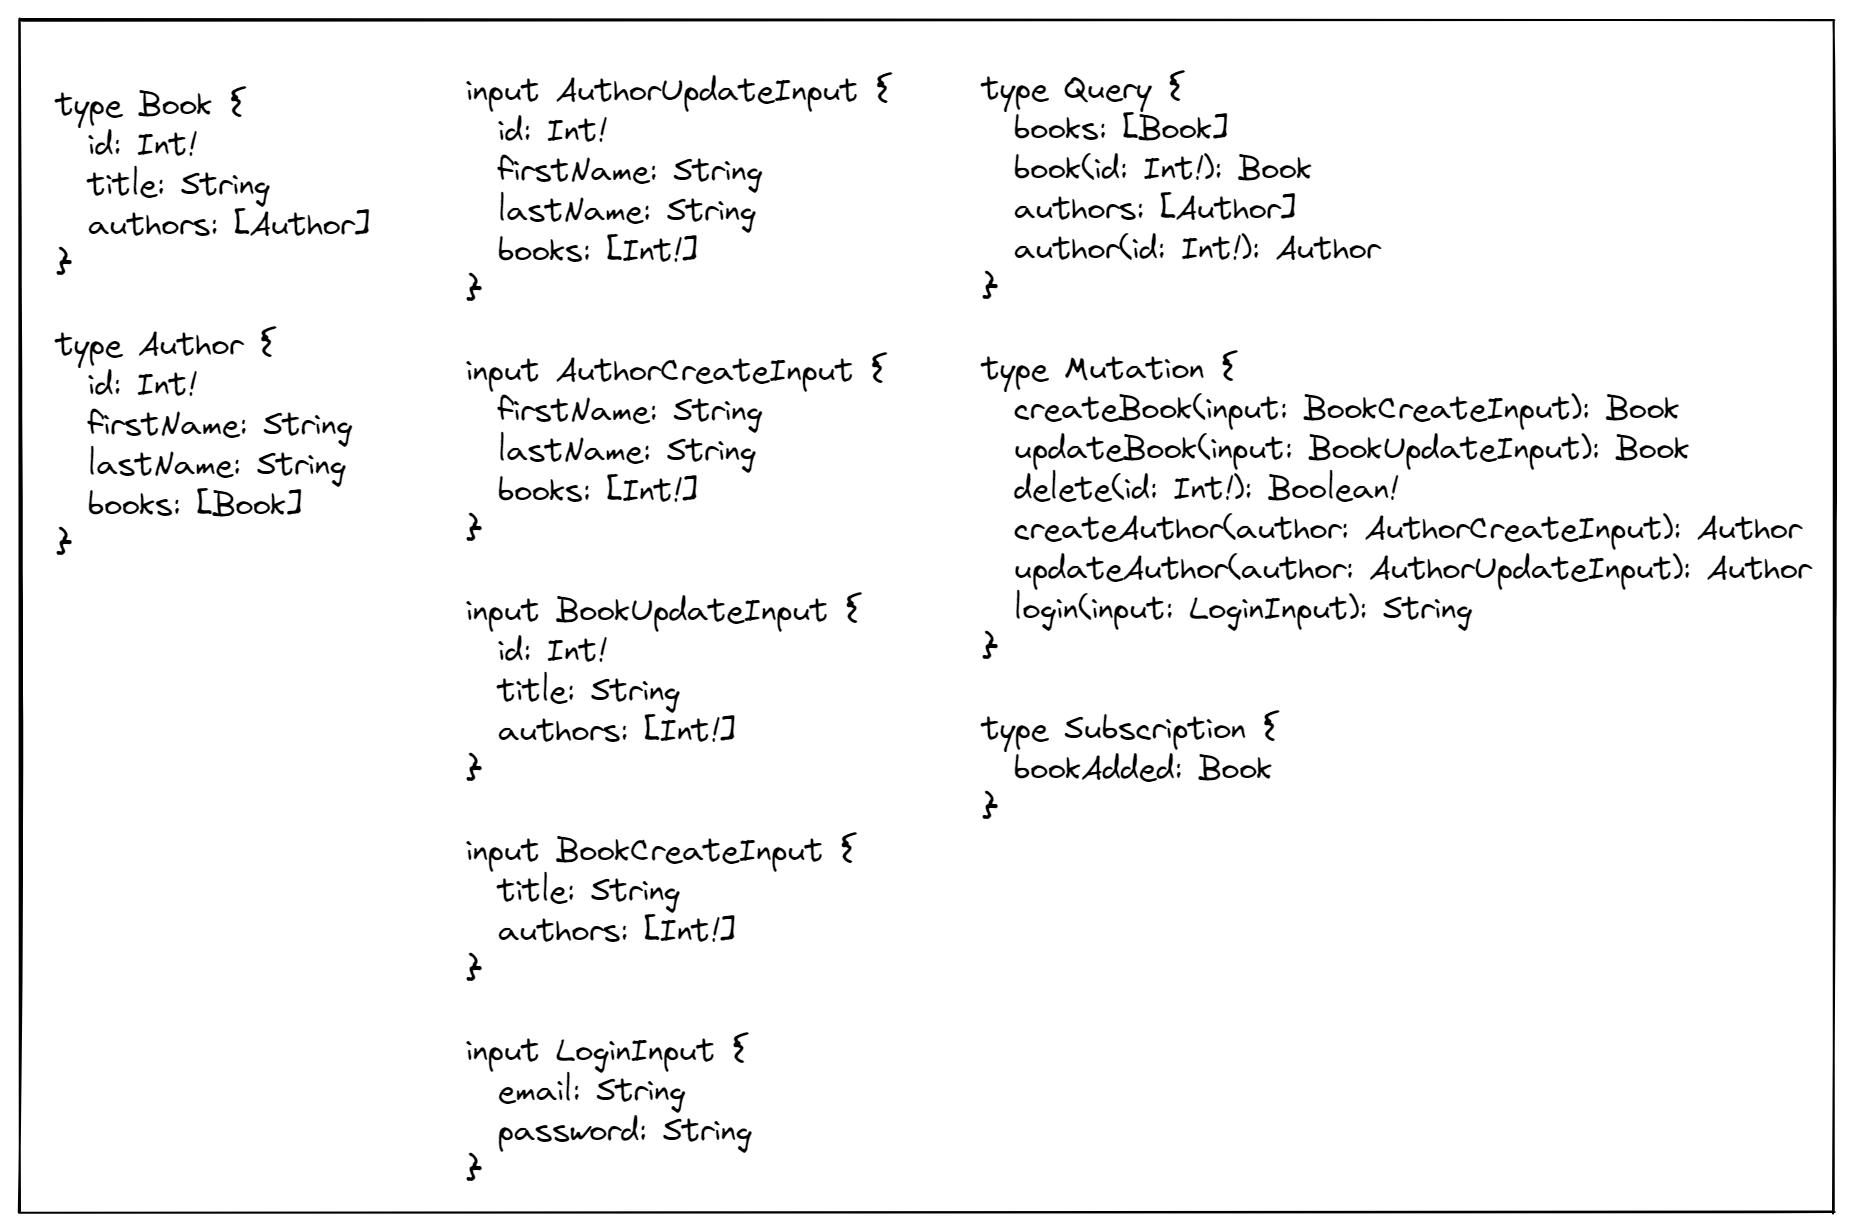
\includegraphics[width=\textwidth]{pics/schema.png}
    \caption{Schemadefinition}
\end{figure}

In Abbildung 3.1 ist eine Schemadefinition zu sehen welche Objekt-Typen, Input-Typen und die Wurzeloperationen beinhaltet.

\section{Parameter}

\section{Lesende und schreibende Zugriffe}
GraphQL liefert keine Spezifikation über die Netzwerkschicht, sondern lediglich eine Empfehlung \textit{HTTP} zu verwenden.
Im Gegensatz zu \textit{REST-APIs} welche bei ihrer Umsetzung \textit{HTTP} verwenden, beschränkt sich GraphQL auf lediglich zwei HTTP-Methoden: GET und POST.
Deswegen ist die Gestaltung und Bennung der Endpunkte nicht so relevant wie bei REST-APIs.
\newline
Der Unterschied, ob ein Client mittels GET oder POST-Anfrage auf den Service zugreift, besteht darin, dass mittels GET-Anfrage nur lesende Zugriffe möglich sind.
Also können mit GET-Anfragen nur Querys aber keine Mutations umsetzen werden.
Desweiteren müsste man jene Query, welche zum Abfragen der Daten verwendet werden sollte, als URL-Parameter übergeben.
Somit gilt es auch zu beachten die Sonderzeichen der Query in \textit{ASCII} umzuwandeln.
Dadurch existiert der Nachteil



% Um schreibend oder lesend auf den GraphQL-Service zugreifen zu können muss an den bereitgestellten Endpunkt eine POST-Anfrage mit einer Query geschickt werden.
% Diese Query ist mittels der \textit{GraphQL Query Language GQL} definiert.
% Eine Anfrage welche eine Query beinhaltet, hat zusätzlich noch zwei optionale Parameter: \textit{variables} und \textit{operationName}.
% Der Name einer Operation wird jedoch nur benötigt wenn mehrere Operationen in der Query auszuführen sind.
% graphql.org/learn/serving-over-http

% Gress Seite 82-83

\section{Querys}

Querys bietet den Clients die Möglichkeit lesend auf die Objekte, welche vom GraphQL-Service verwaltet werden, zuzugreifen.
GraphQL erlaubt es dem Client genau die Daten abzufragen welche er benötigt.
Um auf eine Ressource zuzugreifen wird ein POST-Request an den Wurzelknoten der GraphQL-Applikation geschickt.
Dieser POST-Request enthält ein in der \textit{GraphQL Query Language} definiertes Objekt.
In diesem Objekt werden die auszuführenden Funktionen definiert und welche Felder davon an den Client zu retournieren sind.
Das Ergebnis hat genau jenes Format welches in der Anfrage vom Client definiert wurde.
% Kress 40-41
% \parencite[40]{kress2020graphql}

Da GraphQL mit einem Graphenschema arbeitet, welche auf den Beziehungen der Knoten zueinander basiert, ist es möglich diese Relationen zu nutzen um Daten über mehrere Objekte hinweg zu sammeln.
\newline


In der folgenden Abbildung ist eine verschachtelte Query zu sehen, welche alle Bücher mit den dazugehörigen Autoren anfordert.

\begin{figure}[H]
    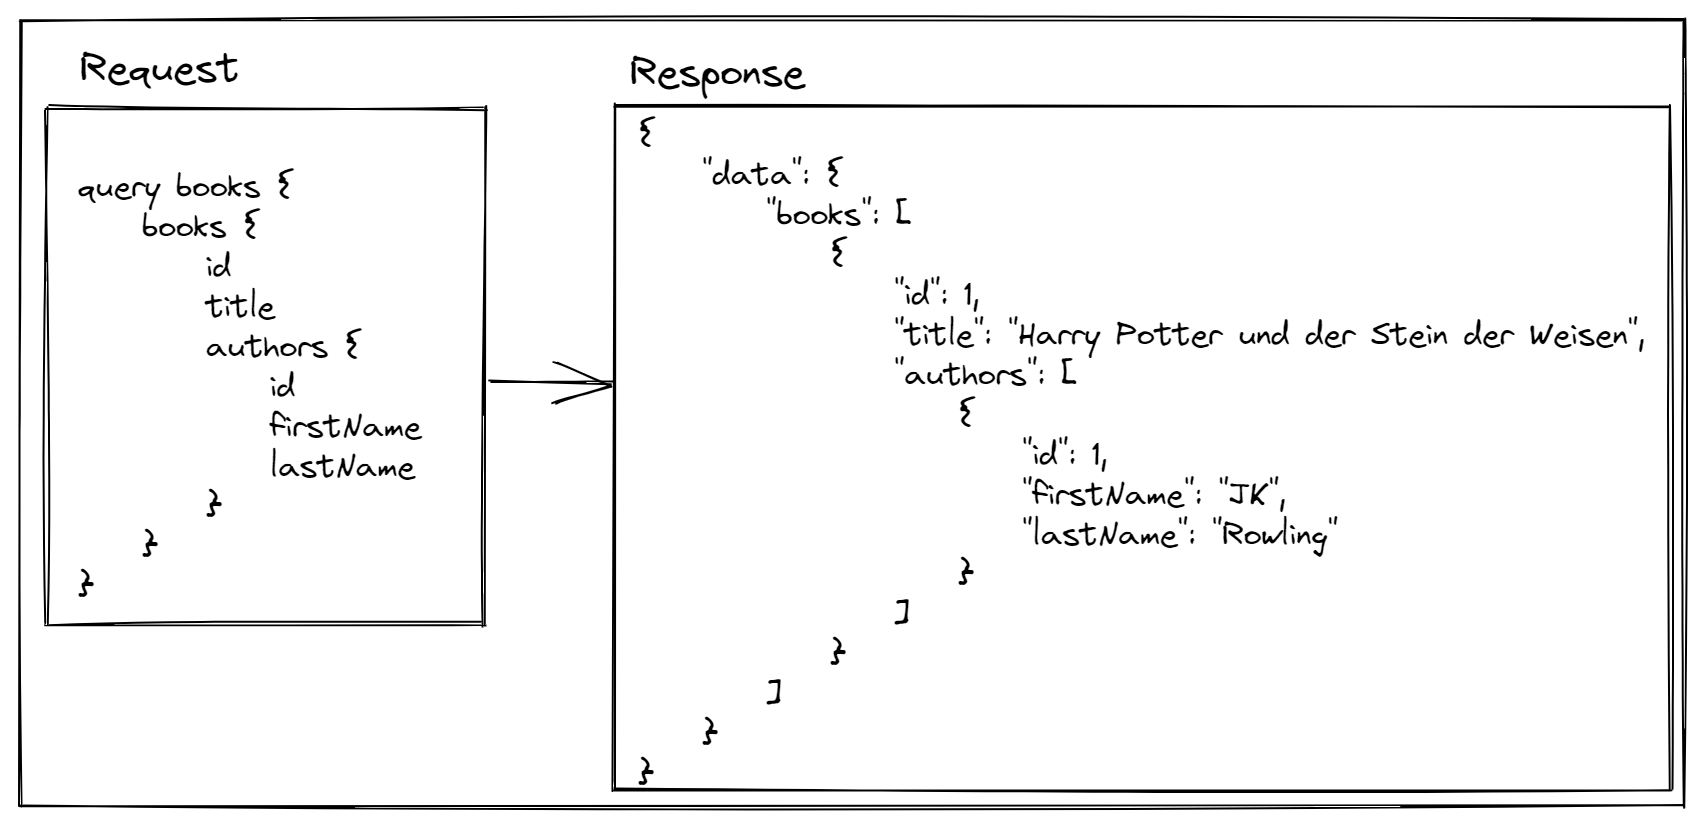
\includegraphics[width=\textwidth]{pics/query_book_with_result.png}
    \caption{Anfrage aller Bücher mit zugehörigen Autoren}
\end{figure}

\subsection{Variablen}
Mit Parametern ist es möglich zusätzliche Daten für spezielle Operationen an den GraphQL-Service zu schicken.
Diese können aber nur statisch in die query eingetragen werden.
Deswegen kann eine GraphQL Operation zudem mit Variablen erweitert werden.
Dadurch hat man verstärkt die Möglichkeit Funktionen wiederzuverwenden.
Variablen müssen am Anfang einer Operation definiert werden und befinden sich während der Ausführung im Lebensraum der Operation.
Diese Variablen werden unter anderem für die Filterung der angeforderten Objekte verwendet.
\newline

In der folgenden Abbildung ist eine Anfrage zu sehen welche das Buch mit der \textit{id = 1} anfordert. Dabei wird die id als Variable übergeben.

\begin{figure}[H]
    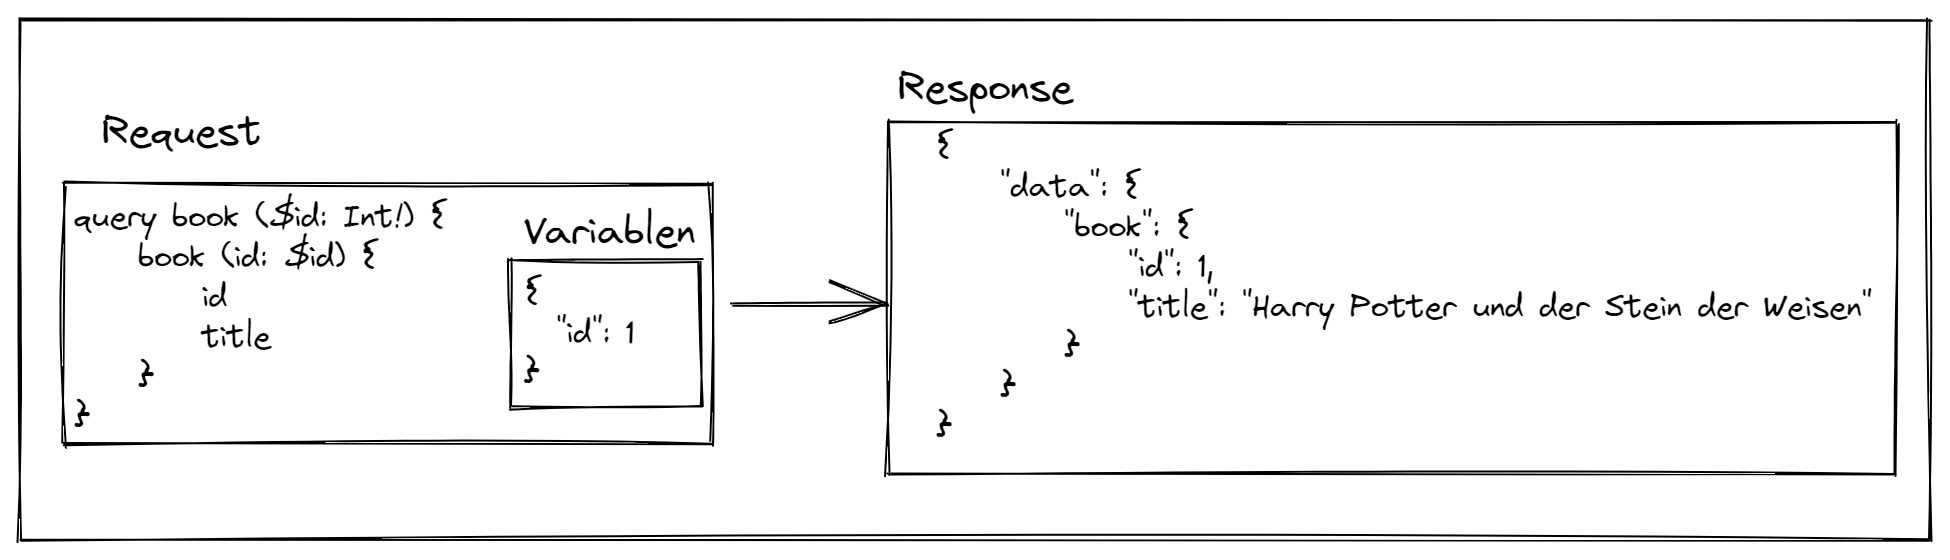
\includegraphics[width=\textwidth]{pics/book_request_with_parameter.png}
    \caption{Anfrage aller Bücher mit zugehörigen Autoren}
\end{figure}

\subsection{Fragmentierung}

\subsection{Aliase}

\section{Mutationen}
APIs benötigen neben dem lesenden Zugriff auf Daten auch einen schreibenden.
Dieser wird in GraphQL mittels Mutationen umgesetzt.
Mutationen kapseln die Implementierungen der Datenbankzugriffsschicht in ein Interface welches die Möglichkeiten zur Manipulation der Daten vorgibt.
Manipulierende Anfragen können Daten dadurch nur auf jene Art und Weise ändern, wie es in der Applikation vorgesehen ist.
% Kress 54

% Mutationen ermöglichen es die Zugriffe 
% Sie werden in der Schemasprache (anderer Begriff ??? -> GDL etc)  mit dem Schlüsselwort mutation definiert.


\subsection{Designempfehlungen}

placeholder
\pagebreak

\section{Bekannte Probleme}

\subsection{Authentifizierung, Autorisierung und Rollenmanagement}

placeholder
\pagebreak

\subsection{1 + n Problem}

\subsection{Subscriptions}

placeholder
\pagebreak

placeholder
\pagebreak

\subsection{Fehlermanagement}

placeholder
\pagebreak

\subsection{Pagination}

\subsection{Caching}

placeholder
\pagebreak
